\section{October 24, 2022}

\subsection{Conjugate stabilizers}

Let $G$ be a group and $S$ be a set. Say that $G$ acts on $S$ by some action. Recall that the set of orbits partition $S$, so 
\[\vert S\vert = \sum_i \vert Gs_i\vert,\]
where $s_i$ are representatives of each orbit.

\begin{theorem}
\proplabel

Stabilizers of points in the same orbit are conjugate.
\end{theorem}

\begin{proof}
\begin{align*}
    \stab_G(gs) &= \{g'\in G : g'\cdot gs = gs\} \\
    &= \{g'\in G : g^{-1}g'g\cdot s = s\},
\end{align*}
which is true if and only if $g^{-1}g'g\in \stab_G(s)$, so $\stab_G(gs) = g \stab_G(s)g^{-1}$.
\end{proof}

\begin{example}
\exlabel

Let $G$ be the rotations of a cube, and $S$ the set of vertices of the cube. 
\end{example}

There's only one orbit, so the stabilizer is always trivial, and therefore every stabilizer is conjugate. 

\begin{example}
\exlabel

Let $G = \RR^2$ act by translation on $S$, the set of horizontal lines. 
\end{example}

The stabilizers are all $\RR\times \{0\}$, which are normal subgroups, so they are conjugate. 

\subsection{Regular Polyhedra}

Let's examine the possibilities for regular polyhedra. A regular polyhedron is defined as a three dimensional geometric solid with identical regular polygons as faces. Let's do casework on the polygon for each face:

\begin{itemize}
    \item Equilateral triangles. When three meet at a vertex, we get a tetrahedron. When four meet at a vertex, we get an octahedron. When five meet at a vertex, we get an icosahedron. We can't have $\geq 6$ meet at a vertex, because six equilateral triangles becomes flat (a regular hexagon).
    \item Square. When three meet at a vertex, we get a cube. We can't have $\geq 4$ for the same reason as before.
    \item Pentagon. When three meet at a vertex, we get a dodecahedron. We can't have $\geq 4$ since $4\cdot 108 > 360$.
    \item Hexagon. We can't have three meet at a vertex, since three hexagons would make a flat surface. Anything larger than a hexagon also won't work.
\end{itemize}

\begin{figure}[h]
\centering
\begin{tabular}{cccc}
\hline
    faces/\# at vertex & 3 & 4 & 5 \\
\hline
    triangle & tetrahedron & octahedron & icosahedron \\
    square & cube & X & X\\
    pentagon & dodecahedron & X & X\\
    hexagon & X & X & X \\
    $\vdots$ & & & \\ 
\end{tabular}
\end{figure}

Thus, there are \ac{5} regular polyhedra in total. Here is a summary:

\begin{figure}[H]
\centering
\begin{tabular}{cccc}
\hline
    & vert. & edges & faces \\
\hline
    tet. & 4&6&4\\
    cub. & 8&12&6\\
    oct. & 6&12&8\\
    icosa. & 12&30&20\\
    dodec. & 20&30&12
\end{tabular}
\end{figure}

Note that the pairs cubes and octahedra, icosahedra and dodecahedra, have the same number of edges, and a swapped number of vertices and faces. We say that these pairs of polyhedra are \ac{dual}, because it is possible to interchange edges and vertices to obtain one from the other. A tetrahedron is said to be dual to itself. In general, dual shapes have the same symmetries. 

\begin{figure}[H]
    \hfill
    \begin{minipage}{0.35\textwidth}
    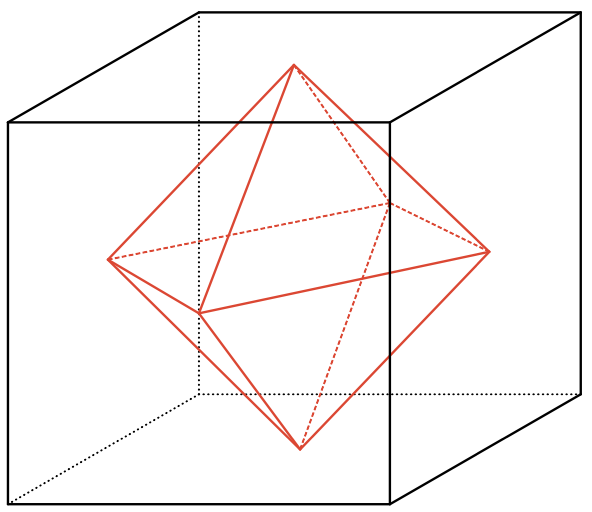
\includegraphics[width=\textwidth]{images/cube_dual.png}
    % \begin{center}\textit{Cube-Octahedron duality}\end{center}
    \end{minipage}
    \hfill
    \begin{minipage}{0.25\textwidth}
    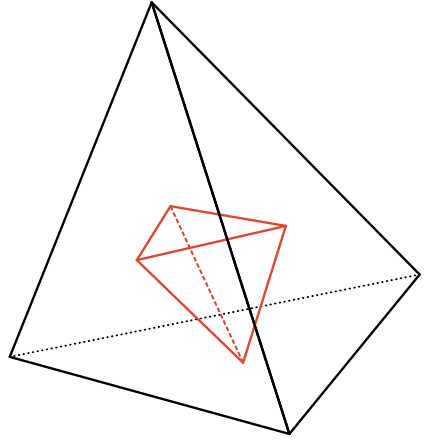
\includegraphics[width=\textwidth]{images/tetr_dual.png}
    % \begin{center}\textit{Tetrahedron-Tetrahedron duality}\end{center}
    \end{minipage}
    \hfill\hfill
\end{figure}\V

\subsection{Finite subgroups of $SO_3(\RR)$}

\begin{theorem}
\thmlabel

Every finite subgroup of $SO_3(\RR)$ is isomorphic to $C_n$, $D_n$, or the rotational symmetries of a platonic solid. 
\end{theorem}

\comment{add proof}
